\documentclass[10pt,letterpaper]{article}
\usepackage{etex}
%\usepackage[utf8]{inputenc}
\usepackage[T1]{fontenc}
\usepackage{amsmath}
\usepackage{amsfonts}
\usepackage{amssymb}
\usepackage{graphicx}
\usepackage{url}
\usepackage{nth}
\usepackage{fixltx2e}
\usepackage{listings}
\usepackage{appendix}
\usepackage{courier}
\usepackage{multicol}
\usepackage{multirow}
\usepackage{adjustbox}
\usepackage[table]{xcolor}% http://ctan.org/pkg/xcolor
\usepackage[htt]{hyphenat}
\usepackage{epigraph}
\usepackage{marginnote}
\usepackage{float}
\usepackage{pgfplots}
\usepackage{pgfplotstable}
\usepackage{tikz}
\usetikzlibrary{shapes,arrows}
\usepackage{draftwatermark}
\usepackage{tabularx,ragged2e,booktabs,caption}
\usepackage{xspace}
\newcolumntype{C}[1]{>{\Centering}m{#1}}
\renewcommand\tabularxcolumn[1]{C{#1}}
\SetWatermarkColor[rgb]{1,0.85,0.85}
\SetWatermarkScale{2.5}
%-------------------------------------------------
% From http://tex.stackexchange.com/a/60212/31317
\usepackage{titlesec}
\usepackage{hyperref}

\titleclass{\subsubsubsection}{straight}[\subsection]

\newcounter{subsubsubsection}
\renewcommand\thesubsubsubsection{\thesubsubsection.\arabic{subsubsubsection}}
\renewcommand\theparagraph{\thesubsubsubsection.\arabic{paragraph}} % optional; useful if paragraphs are to be numbered

\titleformat{\subsubsubsection}
  {\normalfont\normalsize\bfseries}{\thesubsubsubsection}{1em}{}
\titlespacing*{\subsubsubsection}
{0pt}{3.25ex plus 1ex minus .2ex}{1.5ex plus .2ex}

\makeatletter
\renewcommand\paragraph{\@startsection{paragraph}{5}{\z@}%
  {3.25ex \@plus1ex \@minus.2ex}%
  {-1em}%
  {\normalfont\normalsize\bfseries}}
\renewcommand\subparagraph{\@startsection{subparagraph}{6}{\parindent}%
  {3.25ex \@plus1ex \@minus .2ex}%
  {-1em}%
  {\normalfont\normalsize\bfseries}}
\def\toclevel@subsubsubsection{4}
\def\toclevel@paragraph{5}
\def\toclevel@paragraph{6}
\def\l@subsubsubsection{\@dottedtocline{4}{7em}{4em}}
\def\l@paragraph{\@dottedtocline{5}{10em}{5em}}
\def\l@subparagraph{\@dottedtocline{6}{14em}{6em}}
\makeatother

\setcounter{secnumdepth}{4}
\setcounter{tocdepth}{4}
%-------------------------------------------------
\author{Michael Holler}
\title{Automated Textbook Indexing with Na\"ive Bayes Classifier Trained on Wikipedia Articles}
\begin{document}
\maketitle
\newpage
\epigraph{You want weapons? We're in a library! Books! The best weapons in the world! This room's the greatest arsenal we could have---arm yourselves!}{---The Doctor}
\epigraph{Automatic indexing of books has failed miserably, as will be discussed below.}{Nancy Mulvany, {\it Indexing Books}}
\epigraph{The idea behind digital computers may be explained by saying that these machines are intended to carry out any operations which could be done by a human computer.}{---Alan Turing}
\pagebreak
\tableofcontents
\lstset{
	basicstyle=\ttfamily,
	showstringspaces=false,
	numberstyle=\tiny,
	numbersep=10pt,
	numbers=left,
	stepnumber=1,
	frame=single,
	aboveskip=0.5cm,
	belowskip=0.5cm
}
\newpage
\begin{abstract}
Creating the index for a book can be one of two things for an author: arduous, or expensive.
If an automated process can be introduced which effectively generates an index with approximately the same accurracy as a human, it would reduce the time and money authors need to spend on their work, allowing them to allocate those resources in a more useful way.
This preliminary research looks to establish the efficiacy of using a Na{\"i}ve Bayes' classifier trained with data extracted from Wikipedia articles to create an index for a Biology textbook.
The preliminary results suggest that this study's approach is not effective in creating an accurate and effective index.
However the research and results can be used to inform and refine future attempts to automate the indexing process.
\end{abstract}
% Where to put why I decided to use paragraphs for context instead of pages?
\section{Introduction}

The number of books published in the U.S. has been on the rise for at least the past decade, only incurring a small setback in 2005\cite{bowker}.
In 2010, Bowker recorded 328,259 new books published in the United States---up from 302,410 during the previous year.
Despite concerns that the paper book is on it's way out, the book publishing industry is still very much a growing one.

% New Books Published per Year Graph
\begin{center}
\begin{figure}[H]
\label{fig:new-books}
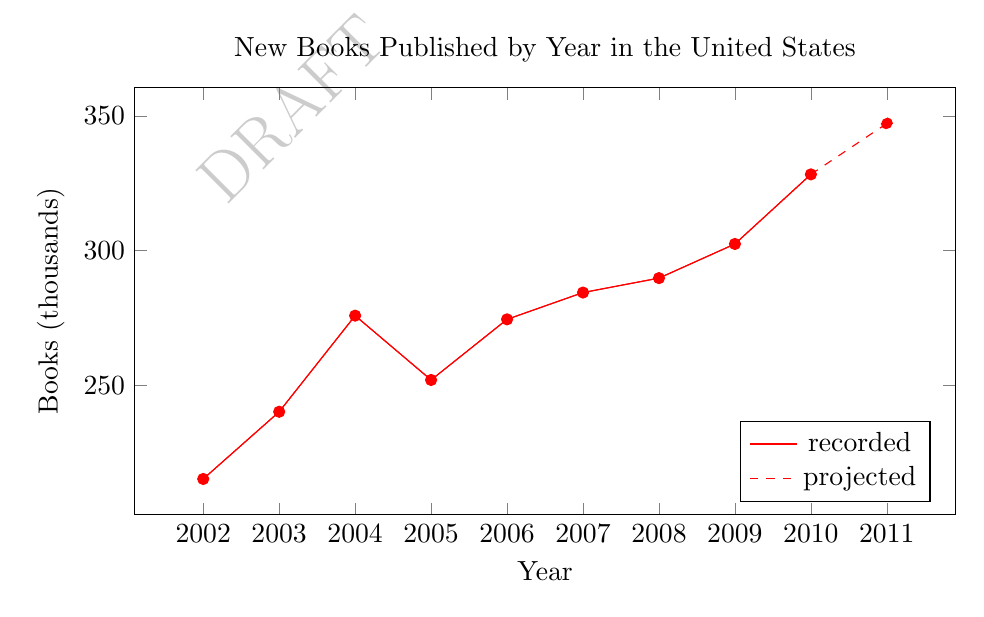
\begin{tikzpicture}
	\begin{axis}[
		title={New Books Published by Year in the United States},
		xlabel={Year},
		xticklabel style={/pgf/number format/1000 sep=},
		ylabel={Books (thousands)},
		width=12cm,
		height=7cm,
		legend pos=south east]
		
		\addplot[color=red,mark=,line join=round, solid] coordinates {
			(2002,215.138)
			(2003,240.098)
			(2004,275.793)
			(2005,251.903)
			(2006,274.416)
			(2007,284.370)
			(2008,289.729)
			(2009,302.410)
			(2010,328.259)
		};
		\addplot[color=red,mark=,line join=round, dashed] coordinates {
			(2010,328.259)
			(2011,347.178)
		};
		\addplot[color=red,mark=*,line join=round, solid] coordinates {
			(2002,215.138)
			(2003,240.098)
			(2004,275.793)
			(2005,251.903)
			(2006,274.416)
			(2007,284.370)
			(2008,289.729)
			(2009,302.410)
			(2010,328.259)
		};
		\addplot[color=red,mark=*,line join=round, dashed] coordinates {
			(2011,347.178)
		};
		
		\addlegendentry{recorded}
		\addlegendentry{projected}
	\end{axis}
\end{tikzpicture}
\caption{Publication statistics for traditional books published in the U.S.\cite{bowker}}.
\end{figure}
\end{center}

It's a fair assumption that many of these new books also contain an index section between their covers.
An index, of course, is, ``An alphabetical list, placed (usually) at the end of a book, of the names, subjects, etc. occurring in it, with indication of the places in which they occur,'' \cite{oed-index}.
Indexes are popular in non-fiction books, particularly in textbooks.
Readers use indexes to quickly and efficiently locate passages of the book focusing on a specific topic.
Thus, it is important for a book's index to be of high quality, so the reader can locate a particular topic with ease.
A good index can make learning and research easy, while a bad index can result in readers' frustration as they scan over each page in an attempt to find what they are looking for.

\subsection{Cost of Indexing}

The growing number of books published each year and the need for quality indexes in books of all types makes indexing an important sub-industry of the publication process.
Since many books contain indexes, any change in the indexing industry directly affects the publication industry.
If indexing could be made more efficient, the publishing industry could allocate the significant resources that would have gone toward indexing to other, more productive areas.

In {\it Indexing Books}, Nancy Mulvany writes that, ``a typical three-hundred-page can easily cost a thousand dollars or more to index.
An example, later in Mulvany's book, estimates a 300 page book at \$1,200.
This was in 2005.
Mulvany goes on to estimate the typical price-per-page at 4--6 2005 U.S. dollars\cite{mulvany}.

The amount of time and money spent on indexing annually can be quantified if a few simplifying assumptions are established.
All rows without citations are conservative guesses for the purpose of estimation:

\begin{center}
\begin{tabular}{|c|l|l|}
\hline
\multicolumn{1}{|c|}{{\bf Symbol}} & \multicolumn{1}{c|}{{\bf Description}} & \multicolumn{1}{c|}{{\bf Statistic}} \\
\hline
$b$ & Number of books published in 2010 \cite{bowker} & 328,259 books \\
\hline
$c$ & Percentage of Books requiring Indexes & 15\% \\
\hline
$d$ & Average dollars per page indexed \cite{mulvany} & \$5 \\
\hline 
$p$ & Average Number of Pages in Book & 300 pgs \\ 
\hline 
$r$ & Average Number of Pages Indexed per Hour \cite{connolly} & 7 pgs/hr \\
\hline
\end{tabular}
\end{center}

Given these variables, equations are developed to calculate average cost and time impact of manual indexing.

\begin{figure}[H]
$$ \text{cost} = b \times c \times p \times d $$
$$ \text{time} = \frac{b \times c \times p}{r} $$
\\
$$ 73,858,275 \text{ USD} = 328259 \times 0.15 \times 300 \times 5 $$
$$ 240 \text{ years}= 2,110,236.48 \text{ hours} = \frac{328259 \times 0.15 \times 300}{7}$$
\caption{The Price of Manual Indexing}
\end{figure}

It is possible to approximate the cost of indexing the 328,259 new books published in 2010 (p.~\pageref{fig:new-books}) by making some conservative assumptions that the average book contains 300 pages, the average price-per-page indexing cost of \$5, and 15\% of books require indexes.
An estimate generated using these numbers reveals that over 70 million dollars were spent on indexing books in 2010. Work hours spent creating indexes is also revealing.

Using a professional indexer's average rate of 7 pages per hour, a similar calculation estimates that over 2 million work hours were spent creating indexes for 2010's new books. It would take a single person 240 years of indexing non-stop.

These numbers reveal the economic impact of indexing, but the individual impact is important too.
If an author wants to index his or her own book, it would take about 42 hours on average. The author could devote an entire work week towards something more productive if there existed an easier way to generate an index.
Clearly, indexing is a significant part of the publishing industry.
Computer software might be able to reduce these high costs, but first it is important to understand the indexing process before computers.

\subsection{Indexing Methods}

Historically, indexing was all done by hand, without the assistance of technology beyond a stack of 3'' x 5'' note cards and a pen.
The ``index card'' method, as it is called, has the indexer create a separate index card for each word or phrase that appears in the index.
These note cards are created on the first pass through the document being indexed, and then they are organized alphabetically.
On the next and subsequent passes, the indexer combs the text looking for references to the words and phrases generated on the first pass, and records each occurrence on the appropriate note card.
At the end of this process, the selection of words and phrases is edited and then typeset \cite{mulvany}.
While this old fashioned method worked in the many years before computers became the powerful productivity tools they are today, computers now help indexers by providing purpose-built software that, in effect, replaces the paper note cards with a more efficient digital representation.

The author of {\it Indexing Books} describes computer-aided indexing by breaking indexing software used into major two types: embedded and dedicated.
Embedded indexing software helps a writer or an indexer mark, in the electronic text itself, the words and phrases that he or she wants to be indexed \cite{mulvany}.
Examples of embedded indexing software are Microsoft Word \cite{ms-word-indexing} and \LaTeX \cite{lamport}.
Dedicated indexing software, on the other hand, only provides tools whose purpose is to make creating an index easier, like the ability to digitize entries, sort them, and structure them in different ways\cite{mulvany}.
Dedicated software is different from embedded because dedicated does not allow the user to modify or display the full text of the work itself, instead focusing only on the index.
Examples of dedicated software are Macrex\cite{macrex} and SKY Index Professional\cite{sky-software}.
While these two types of software help people generate indexes, it is not the type of software this research is concerned with.

Automatic indexing is the lesser known third type of indexing software, and it is the subject of this research.
Mulvany defines automatic indexing software as that which, ``conjures up images of indexing at the push of a button, the computer taking care of all the drudgery and the thinking involved in creating an index''\cite{mulvany}.
Although she recognizes it as a computer science research focus, she does not think highly of present-day automatic indexing, stating that, ``There is nothing automatic about the index-writing process.
There is no automatic indexing tool available that could produce the index in the back of this book''\cite{mulvany}.
Given the career implications of automatic indexing on indexing professionals, it is unsurprising that Mulvany is skeptical.
However, for the most part she is correct: current software does not perform as well as humans at the task of indexing a book.
If it did perform better than humans, than publishers and authors would be purchasing the software rather than hiring indexers.

The goal of this research is to further the knowledge of automatic indexing by applying techniques from Natural Language Processing (NLP), a subfield of Computer Science that concerns itself with teaching computers to understand language mechanics.
The next section takes a brief look at what Natural Language Processing is, and how it pertains to indexing.

% TODO: Explain/preview structure of paper.



\section{Background}
% Background section placeholder (move everything below this to another file eventually).
The process of creating an index is either costly or time consuming for authors, depending on whether they choose to create the index themselves or pay someone to do it.
The act of creating an index is labor and organization intensive, often requiring a text to be read multiple times while keeping track of entries electronically or on index cards.

Given that indexing a book is so expensive and time consuming, it makes sense to see if computers can be used to generate an index that is nearly as accurate as human indexers.
To automate the indexing process, software exists to replace the indexer's index cards with a more efficient computerized organization system.
However, there is a new, rising interest in seeing if computers can generate indexes deterministically, without the help of human beings.
To do this, software engineers and researchers must apply natural language processing techniques in new and interesting ways.

\subsection{Indexing Process}
% How humans create indexes today.


Although statistics on the number of books that have indexes or the number new textbooks per year do not appear to exist, it seems a safe assumption to 

\subsection{Natural Language Processing}
\section{Data Collection}
\label{sec:data-collection}

This research leverages supervised learning algorithms, meaning it requires a training set and a test set to develop an appropriate feature set to use in conjunction with the supervised learning algorithm.
The training set allows the document classifier to ``learn'' how to classify different sections of text, and the test set is used to validate that documents are classified correctly.

Generally, training and test data come from the same corpus, the same set of data~\cite{jurafsky}.
This research takes test and training set data from two different, mutually exclusive corpora.
The reason for this deviation for convention is to answer the question of whether Wikipedia data can be used to train for any more specific set of input data, like paragraphs from a Biology textbook.
The training set is composed of paragraphs from Wikipedia articles, with each paragraph labeled by the title of the article it belongs to.
The test data contain paragraphs from the OpenStax {\it Biology} textbook~\cite{biology}, with each paragraph labeled by the index entry that refers to it.\footnote{If a {\it Biology} paragraph is not referenced in the index, it is not included in the data set. If it is referenced by multiple index entries, the paragraph is included once per index entry.}

Due to the sheer size of Wikipedia and the memory and computational power available for this research, the data set was reduced by selecting only paragraphs from Wikipedia articles whose title matched an index entry in {\it Biology}.
Likewise, this research makes an assumption that the set of all reasonable index entries for any textbook is the same as the set of all titles in the English Wikipedia.
This assumption lends itself to selecting only paragraphs from {\it Biology} whose labels are the same as Wikipedia article titles.

The following sections contain justification for the choice of data for each set, and the methods used to structure and collect that data for analysis.

\subsection{Data Collection Pipeline}

The data for both the training and test sets are collected in a generally similar fashion.
The source data is parsed and placed into a relational database described in Appendix~\ref{appendix:a}.
This relational database is used to make extracting information from both texts and comparing the two data sets easier.

Since writing the Python NLTK \naive Bayes classifier is much easier if the data can be extracted directly from files (rather than by connecting to the relational database), data are extracted from the relational database and stored into plain text files.
Text in these files are separated into paragraphs by a double newline ({\tt \textbackslash n\textbackslash n}).
Figure~\ref{fig:pipeline} visually depicts the pipeline described above.

% Define block styles
\tikzstyle{block} = [rectangle, draw, 
    text width=5em, text centered, rounded corners, minimum height=4em]
\tikzstyle{line} = [draw, -latex']

\begin{figure}[H]
\begin{center}
\begin{tikzpicture}[node distance = 3cm, auto]
    % Place nodes
    \node [block] (source) {source data};
    \node [block, right of=source] (relational) {relational database};
    \node [block, right of=relational] (files) {plain text files};
    % Draw edges
    \path [line] (source) -- (relational);
    \path [line] (relational) -- (files);
\end{tikzpicture}
\caption{The data collection pipeline.}
\label{fig:pipeline}
\end{center}
\end{figure}

In order to move data from one section of the data collection pipeline to another, custom scripts were created to automate the process.
All scripts mentioned in this paper without citation were created specifically for this research by the author.
The source code for these scripts, as well as the data used in the research, are freely available online (see Appendix~\ref{appendix:c}).

\subsection{Training Set}
\label{subsec:training-set}

The training set is created from a list of Wikipedia articles whose titles are also index labels in {\it Biology} (see section~\ref{subsec:reducing}).
Since this list contains only titles, the contents of the article need to be fetched from Wikipedia itself.

\subsubsection{Downloading the Training Data}

There are numerous articles to fetch from Wikipedia (see section~\ref{subsec:reducing}).
Downloading each one-by-one would take time and violate Wikipedia's terms of service. Wikipedia does not allow the use of automated web crawlers when it can be avoided~\cite{wiki-robots}.

Instead, the articles were fetched using the Wikipedia page exporter~\cite{wiki-exporter}, which produces an XML database dump file.
This file contains the textual contents of all the articles specified in the web form, plus extra information about the article like title and date of last edit.
The contents of the article are stored in the MediaWiki markup language~\cite{mediawiki-markup}.
This language works similarly to other markup languages like HTML and Markdown, and is used everywhere on Wikipedia.
Using the page exporter makes it possible to circumvent Wikipedia's rules about crawling the website because the export happens in one bulk data transfer rather than the many very small and frequent transfers a web crawler would make.

Wikipedia content editors must use the MediaWiki markup language to edit pages. 
While MediaWiki markup is great for writing and editing content, it is difficult for computers to directly query text written in the language.
To solve this problem, the MediaWiki format may be converted to HTML.
HTML has the useful {\tt <p>} tag, which is used to distinguish paragraphs from one another, a requirement for this research. 
Unfortunately, the only full-featured MediaWiki markup to HTML converter is part of Wikipedia itself.
Thankfully, Wikipedia runs on the MediaWiki framework, which is a free, open source application used to host Wikis in the same way that Wordpress is a platform that hosts blogs.
The file that was created in the page exporter step above can be imported into any hosted MediaWiki installation, even one on a personal computer.
By installing MediaWiki on a personal computer and importing the database export file from Wikipedia, one can create their own miniature version of Wikipedia that contains only the articles one is interested in.

\subsubsection{Converting MediaWiki Markup to HTML}

To convert the exported articles to HTML, a local MediaWiki server was installed on a personal computer using MediaWiki's online instructions~\cite{mediawiki-installation} with the purpose of creating a local version of Wikipedia that only contains the articles that share titles with index labels from {\it Biology}.
This mini-Wikipedia can then be crawled using printPageLinks.py to extract and store the HTML versions of the articles.

After installation, all available first-party MediaWiki plugins were enabled in the installation, as Wikipedia uses many of them on their own MediaWiki installation.
Once installed, the database import tool~\cite{mediawiki-import} was used to import the XML file from Wikipedia's database dump into the local MediaWiki installation, creating a small version of Wikipedia containing only the articles needed for this research.
The MediaWiki platform takes care of converting MediaWiki markup into HTML when it receives an HTTP request for a given article, just like regular Wikipedia.

\subsubsection{Finding Redirects}
\label{subsec:finding-redirects}

Inspection of the articles imported into the local MediaWiki installation showed that a large number of the articles are actually just redirect pages to a complete article with a different name.
The Wikipedia exporter does not provide the full pages the redirect pages reference.
There is, however, a way to obtain a list of the full-text files.
Here is an example of what a redirect page looks like in the XML database dump:

\begin{lstlisting}
<page>
  <title>5' cap</title>
  <ns>0</ns>
  <id>37542765</id>
  <redirect title="Five prime cap" />
  <revision>
    <id>528722171</id>
    <parentid>521385832</parentid>
    <timestamp>2012-12-19T00:45:42Z</timestamp>
    <contributor>
      <username>MZMcBride</username>
      <id>212624</id>
    </contributor>
    <minor/>
    <comment>[[bugzilla:42616]]</comment>
    <text xml:space="preserve" bytes="28">
        #REDIRECT [[Five prime cap]]
    </text>
    <sha1>kzecsgfge2ind0a0652k24ldw1unbgd</sha1>
    <model>wikitext</model>
    <format>text/x-wiki</format>
  </revision>
</page>
\end{lstlisting}

Line 5 in the above sample shows a redirect tag that contains the title of the complete article this page redirects to.
These redirect tags were discovered by using findRedirects.py.
This script does two things.
First, it changes the {\tt wikiTitle} field in the {\tt indexToWiki} table from the title of the redirect page (``$5^\prime$ cap'' in the above example) to the title of the page it redirects to (``Five prime cap``).
Second, it prints out the wikified title (``Five prime cap'' becomes ``Five\_prime\_cap``) on each line of output.
The results of the program's output were then copy-pasted back into the Wikipedia exporter~\cite{wiki-exporter}, yielding a new XML database dump full of the complete articles.
This XML file was then imported into the MediaWiki site, giving the redirect pages their respective targets to point to.

The process of resolving redirects did not need to be done on the second XML database dump because it only contained full articles (no redirects to other pages).

\subsubsection{Saving Pages as HTML}
\label{sec:html-pages}

Once all necessary articles were imported into the local MediaWiki server, it became possible to download them all in HTML.
To do this, a list of links to each of the articles imported into the MediaWiki server was required.
MediaWiki provides this list via the {\tt Special:AllPages} family of pages.
printPageLinks.py was used to locate all of the links on these special pages and download all non-redirect articles in HTML.
The Python script saves each article in a file with the same title as the article itself.

\subsubsection{Extracting Paragraphs from Article HTML}
\label{sec:training-files}

Once the articles were made accessible in HTML, the paragraphs needed to be extracted from these articles and stored in the same format as the {\it Biology} paragraphs from section~\ref{subsubsec:RDB2F}.
Another Python tool---html2text.py---used BeautifulSoup~\cite{beautifulsoup} to extract the contents of all {\tt <p>} tags from the body of each HTML Wikipedia article.
The script appends each paragraph to a file (one file per article) with each paragraph in the file separated by two newline characters as in section~\ref{subsubsec:RDB2F}.

\subsubsection{Dealing with Disambiguation Pages}

Redirect pages are not articles in and of themselves, so they were removed from the training set.
However, there is also another type of article whose content does not accurately represent a specific concept, and those are disambiguation pages.

\begin{quote}
Disambiguation in Wikipedia is the process of resolving the conflicts that arise when a single term is ambiguous---when it refers to more than one topic covered by Wikipedia.~\cite{wiki-disambiguation}
\end{quote}

A disambiguation page differs in content from a redirect page in two primary ways: disambiguation pages do not follow a specific structure and always link to more than one page.
Since the subjects of disambiguation pages are, by nature, multi-topic, they should not be used for this research.

Disambiguation pages are difficult to locate and remove because they do not follow a specific structure, although they are fairly obvious to the human eye.
Thus, disambiguation pages were removed with the help of cullDisambiguation.sh, a script which displays an article to the user and asks them whether it should be kept or deleted.

Although there was not a deterministic process guiding script, articles were only deleted if they contained sentences in the article ``abstract'' following the patterns, ``X commonly refers to,'' ``Y may also refer to'' or similar. Articles are also considered to be disambiguation pages if they contained unordered lists of links to similarly named articles.

\subsubsection{Removing Spurious Article Text}

Several of the plain text paragraph files contain spurious ``paragraphs'' at the end of the file which are either ``Cite error''s or links to view the article in a different language.
Neither of these traits are relevant to the article, so they were safely removed.
Unlike disambiguation pages, locating and removing these errors followed a deterministic, repeatable process.
The offending pages were located using the pattern matching script cullSpuriousArticleText.sh and the spurious text was manually removed from each article found this way.
Manually deleting the spurious lines prevented false positive matches from being removed from the articles, since this text could conceivably (however unlikely) appear in-context within the text of an article.

\subsubsection{Discovering Most Commonly Linked Articles}
\label{sec:ranked-titles}

During analysis, (see section~\ref{subsubsubsec:feature-links}), it was deemed useful to create a list of Wikipedia article titles that are linked to in the training set of Wikipedia articles, ranked most-linked-to first.
It is important to remember that the title of a linked Wikipedia article is not necessarily the same as the title of the linked text that the user may click on to visit the linked article.

An example of this is shown in a piece of HTML excerpted from the Biology article, which displays ``branches and subdisciplines'' to the user, but actually links to the article titled ``List of biology disciplines'':
\begin{lstlisting}[language=HTML]
<a href="/wiki/List_of_biology_disciplines"
   title="List of biology disciplines"
   class="mw-redirect">branches and subdisciplines</a>
\end{lstlisting}
\noindent For the purpose of this research, the contents of the title attribute were extracted and ranked by most frequently linked.
These titles were pulled from the ``a'' link elements in the HTML versions of the Wikipedia pages mentioned in section~\ref{sec:html-pages} by using extractPageLinks.py to generate a rankedTitles.txt file.

\subsection{Test Set}
\label{subsec:test-set}

Since the goal of this research is to create an index for a book, the test set was generated from a textbook with a comprehensive index section.
This textbook is called {\it Biology}~\cite{biology}, and is freely available from OpenStax~\cite{openstax-bio} under the Creative Commons Attribution license.
The book was created by six senior contributors that hold professorial positions at prestigious universities, and approximates an average college textbook.
This textbook is 1,477 pages long, containing an index of 3,118 unique topics (labels) making for 4,678 different index entries (references).

In {\it Biology}, all words referred to by index entries are bolded in the text itself. Below is an example of what this looks like (bold in original):

\begin{quote}
Symbiotic relationships, or {\bf symbioses} (plural), are close interactions between individuals of different species over an extended period of time which impact the abundance and distribution of the associating populations.~\cite{biology}
\end{quote}

\noindent Here, the bold word ``symbioses'' is referred to by an index entry at the back of the book with the same name. All index entries point to bold words, and all bold words point to index entries. This fact makes it trivial to find which part of the page an index reference is referring to, making it a good candidate for test data.

\subsubsection{Structuring the Test Data}

Useful though {\it Biology} is as a data source, it is not available in a structured, easily parsable format.
In order to make the data in {\it Biology} usable, it was converted from its source PDF into a structured form.
A relational database was used to store the book's text so that it can be queried for its contents, paragraph location, page number, and other helpful attributes.

\subsubsection{Importing Index Entries into Relational Database}

To expedite the structuring process, text was copied manually from the PDF, and pasted into a plain text document.
Regular expressions were used to massage the data into a simple, comma separated format.
In this format, each line represents a unique index entry, with the first column in a line holding the index label (or name), and each subsequent column holds a page number the label can be found on.

A table was created to hold the index labels separate from the page numbers, since one label can refer to multiple pages.
In this table, indexId is an autoincrementing ID, label is the name of the index entry as it appears in the book (e.g., ``Acid rain''), and wikiLabel is the label if the label were a wikipedia article name (e.g., ``Acid\_rain'') which is achieved by replacing spaces in the label with underscores.

\begin{center}
\begin{tabular}{|c|}
\hline 
\textbf{index} \\ 
\hline 
bookId \\ 
\hline 
indexId \\ 
\hline 
label \\ 
\hline 
wikiLabel \\ 
\hline 
\end{tabular}
\end{center}
 
An indexedPage table was created to store index references (page numbers) that belong to index labels.
This table simply contains an indexId and a pageNum, which allows for joins onto the index table to replicate the whole index.

\begin{center}
\begin{tabular}{|c|}
\hline 
\textbf{indexedPage} \\ 
\hline 
indexId \\ 
\hline 
pageNum \\ 
\hline 
\end{tabular} 
\end{center}

Once these tables were created, the structured CSV file was imported using the custom indexImporter.php tool written specifically for this purpose.

The importer script populates all of the columns in both tables with all of the data in the CSV file.

\subsubsection{Reducing Index Entry Set}
\label{subsec:reducing}

Only index entries whose {\tt wikiLabel} value matches a Wikipedia article title will be used in this research.
This means that information need only be gathered from index entries that match this criteria.
To discover this subset of index entries, a database of Wikipedia titles must be intersected with the {\tt index}.

The Wikimedia Foundation periodically creates dumps for their many databases and makes them publicly available online~\cite{wiki-dumps}.
One of the many data sets they make available is a list of Wikipedia article titles in the main {\tt /wiki/} namespace for the English language version of Wikipedia~\cite{wiki-dump-titles}.
At the time of this writing, there are 10,639,771 separate Wikipedia article titles matching this criteria.
This dump will serve as the source that will ultimately be intersected with the {\it Biology} index entries to yield the entries that will be used in analyses.

Before performing this intersection, the English Wikipedia title information must be extracted from the dump file and placed in a table in the relational database.
This table contains a unique {\tt titleId} integer key and a textual {\tt title} in each row.

\begin{center}
\begin{tabular}{|c|}
\hline 
{\bf articleTitles} \\ 
\hline 
titleId \\ 
\hline 
title \\ 
\hline 
\end{tabular} 
\end{center}

This data was imported into the {\tt articleTitles} table using the titleImporter.php script.
With both the index labels and article titles in the relational database, the two data sets were intersected by running the following MySQL command ({\tt BINARY} requires case sensitive matching):

\begin{lstlisting}[language=SQL]
SELECT i.wikiLabel
    FROM `index` i, `articleTitles` at
    WHERE BINARY i.wikiLabel = at.title;
\end{lstlisting}

The 3,118 unique index labels intersected against all 10,639,771 Wikipedia articles yields a total number of 518 overlapping terms.
This number was so low because all Wikipedia titles begin with a capital letter, but not all index labels did, even if the word was not a proper noun or acronym.
Since this selection was restricted to exact case matches only, all index labels with lowercase initial letters were excluded from the intersection.
This does not seem to introduce a bias towards proper nouns, however, as {\it Biology}'s index contains words and phrases exactly as they appear in the text.
Below is a random sampling of 15 labels from the intersection as they appear in {\it Biology}'s index.
Notice how very few of these labels are proper nouns.

\begin{multicols}{3}
\begin{verbatim}
Bacteriophages
Chordata
Elevation
Exotic species
FtsZ
Heritability
Phloem
Pongo
RNAs
Runners
Schwann cell
S-layer
Southern blotting
Sutural bones
Topoisomerase
\end{verbatim}
\end{multicols}

\subsubsection{Storing the Indexed Text}

Now that the relevant set of index labels have been ascertained, the context in which these labels appear in {\it Biology}'s text must be stored.
As mentioned above, this research defines an index entry's context as the paragraph the indexed word appears in.
In the relational database, two tables exist to hold this information:

\begin{center}
\begin{tabular}{|c|}
\hline 
\textbf{paragraph} \\ 
\hline 
paraNum \\ 
\hline 
bookId \\ 
\hline 
pageNum \\ 
\hline 
endPageNum \\ 
\hline 
body \\ 
\hline 
\end{tabular}
\end{center}

\begin{center}
\begin{tabular}{|c|}
\hline 
\textbf{indexedParagraph} \\ 
\hline 
indexId \\ 
\hline 
paraNum \\ 
\hline 
\end{tabular} 
\end{center}

The contents of a paragraph are stored in the {\tt paragraph} table's body, along with information about the paragraph's location.
{\tt pageNum} and {\tt endPageNum} specify the pages on which the paragraph starts and ends, since a paragraph may continue onto another page.

To associate these paragraphs with the index labels in the {\tt index} table, the indexedParagraph table was created.
This lookup table specifies a many to many relationship between {\tt paragraph} and {\tt index}, since an index entry refers to at least one paragraph, and a paragraph may contain zero or more index references. Once these tables were created, the text from {\it Biology} could be extracted from the source PDF and imported into the database.

\subsubsection{Collecting the Indexed Text}

The paragraphs were imported into the relational database using paragraphImporter.php, a small webpage script written specifically for this purpose, allowing a researcher to copy a paragraph into a textbox on that page and fill in the meta data for that paragraph and keep track of the index entries that point to it.

As mentioned above, {\it Biology} comes in PDF form, making it difficult for a computer to parse out the individual paragraphs.
By using the SQL query below, a list of index entries with the pages on which they appear is extracted from the database.

\begin{lstlisting}[language=SQL]
SELECT DISTINCT ip.pageNum, i.`label`
    FROM thesis.`index` i,
         thesis.indexToWiki iw,
         thesis.indexedPage ip
    WHERE BINARY i.`label` = iw.indexTitle
        AND ip.indexId = i.indexId
        ORDER BY ip.pageNum ASC;
\end{lstlisting}

This list is used to guide data entry, since it contains only the index references which are relevant for this research.
Here is an example of what this list looks like:

\begin{multicols}{2}
\begin{verbatim}
14,Science
16,"Deductive reasoning"
16,"Inductive reasoning"
20,"Basic science"
23,"Review articles"
27,Organs
27,Prokaryotes
28,Organisms
32,Microbiology
33,Zoology
\end{verbatim}
\end{multicols}

Using this list and a PDF viewer, a paragraph is located that corresponds to each line, the text is selected using the cursor, and copied from the PDF to paragraphImporter.php.
Finding which paragraph on a page corresponds to a given index label is a trivial task, as the label always appears bolded in the paragraph it belongs to.

\subsubsection{Relational Database to Files}
\label{subsubsec:RDB2F}

This research uses Python's Natural Language Toolkit (NLTK) library for analysis~\cite{nltk}.
With NLTK, it is easier to work with raw files without interacting with a database.
In order to do this, the content that was inserted into the database in the above step needs to be extracted.
The extraction is accomplished using saveIndexParagraphs.php, a script which connects to the database and places paragraphs in files named by their respective index labels.
All of the paragraphs a label refers to are appended to the same file, using two newline characters ({\tt{\textbackslash}n{\textbackslash}n}) as a delimiter between paragraphs.
It is also important to note that a paragraph will be placed in multiple files if multiple labels refer to it.
Now the test set is considered processed, it is time to move on to the training set.

\subsection{Mapping the Training Set to the Test Set}
\label{sec:indexToWiki}

Before discovering that some of the Wikipedia articles were actually empty redirect pages as discussed in section~\ref{subsec:finding-redirects}, there was thought to be a direct mapping between {\it Biology} index labels and Wikipedia articles.
Afterwards, it was established that the link between an index label and its article may be transitive through redirect pages.
The section maintained a mapping from index label from Wikipedia article in the indexToWiki table by resolving page redirects.
Although this information is stored in the relational database, it is easier to make use of the data if it exists in an easily portable file, rather than a more difficult to move database.
This makes it easy to distribute the analysis portion of the research using commodity hardware offline.
Therefore, a CSV copy of this mapping was created using the following SQL call:
\begin{lstlisting}[language=SQL]
SELECT indexTitle, wikiTitle FROM thesis.indexToWiki;
\end{lstlisting}
\noindent Since the size of the resulting indexToWiki.json was reasonably small, the file was converted to JSON by hand using vim and regular expressions.

Once of the data were collected, parsed, and organized, the analysis of the data and attempt at automatically regenerating {\it Biology}'s index could begin.

\section{Analysis}

% Results including Number of Samples.
% Please remember to add \use{multirow} to your document preamble in order to suppor multirow cells
%\begin{table}[h]
%\begin{tabular}{cllll}
%\hline
%\multicolumn{1}{l}{\textbf{\begin{tabular}[c]{@{}c@{}}Number of \\ Samples\end{tabular}}} & \textbf{Sensitivity}               & \textbf{Feature}                        & \textbf{Sampling Technique} & \textbf{Accuracy} \\ \hline
%\multirow{24}{*}{2000}                                                                    & \multirow{12}{*}{Case-sensitive}   & \multirow{3}{*}{Contains}               & Least frequent              & 0.20\%    \\ \cline{4-5} 
%\multicolumn{1}{l}{}                                                                      &                                    &                                         & Most frequent               & 0.13\%   \\ \cline{4-5} 
%\multicolumn{1}{l}{}                                                                      &                                    &                                         & Random                      & 0.20\%    \\ \cline{3-5} 
%\multicolumn{1}{l}{}                                                                      &                                    & \multirow{3}{*}{In first sentence}      & Least frequent              & 0.20\%    \\ \cline{4-5} 
%\multicolumn{1}{l}{}                                                                      &                                    &                                         & Most frequent               & 1.82\%    \\ \cline{4-5} 
%\multicolumn{1}{l}{}                                                                      &                                    &                                         & Random                      & 0.20\%    \\ \cline{3-5} 
%\multicolumn{1}{l}{}                                                                      &                                    & \multirow{3}{*}{First word in sentence} & Least frequent              & 0.20\%    \\ \cline{4-5} 
%\multicolumn{1}{l}{}                                                                      &                                    &                                         & Most frequent               & 0.61\%   \\ \cline{4-5} 
%\multicolumn{1}{l}{}                                                                      &                                    &                                         & Random                      & 0.40\%    \\ \cline{3-5} 
%\multicolumn{1}{l}{}                                                                      &                                    & \multirow{3}{*}{Linked article titles}  & Least frequent              & 0.20\%    \\ \cline{4-5} 
%\multicolumn{1}{l}{}                                                                      &                                    &                                         & Most frequent               & 1.21\%    \\ \cline{4-5} 
%\multicolumn{1}{l}{}                                                                      &                                    &                                         & Random                      & 0.40\%    \\ \cline{2-5} 
%\multicolumn{1}{l}{}                                                                      & \multirow{12}{*}{Case-insensitive} & \multirow{3}{*}{Contains}               & Least frequent              & 0.20\%    \\ \cline{4-5} 
%\multicolumn{1}{l}{}                                                                      &                                    &                                         & Most frequent               & 0.14\%   \\ \cline{4-5} 
%\multicolumn{1}{l}{}                                                                      &                                    &                                         & Random                      & 0.40\%    \\ \cline{3-5} 
%\multicolumn{1}{l}{}                                                                      &                                    & \multirow{3}{*}{In first sentence}      & Least frequent              & 0.20\%    \\ \cline{4-5} 
%\multicolumn{1}{l}{}                                                                      &                                    &                                         & Most frequent               & 3.03\%     \\ \cline{4-5} 
%\multicolumn{1}{l}{}                                                                      &                                    &                                         & Random                      & 0.20\%    \\ \cline{3-5} 
%\multicolumn{1}{l}{}                                                                      &                                    & \multirow{3}{*}{First word in sentence} & Least frequent              & 0.20\%    \\ \cline{4-5} 
%\multicolumn{1}{l}{}                                                                      &                                    &                                         & Most frequent               & 0.61\%   \\ \cline{4-5} 
%\multicolumn{1}{l}{}                                                                      &                                    &                                         & Random                      & 0.40\%    \\ \cline{3-5} 
%\multicolumn{1}{l}{}                                                                      &                                    & \multirow{3}{*}{Linked article titles}  & Least frequent              & 0.40\%    \\ \cline{4-5} 
%\multicolumn{1}{l}{}                                                                      &                                    &                                         & Most frequent               & 9.49\%    \\ \cline{4-5} 
%\multicolumn{1}{l}{}                                                                      &                                    &                                         & Random                      & 0.40\%    \\ \hline
%\end{tabular}
%\end{table}

% Please remember to add \use{multirow} to your document preamble in order to suppor multirow cells
\begin{center}
\begin{table}[h]
\caption{Indexing results using 2000 features.}
\begin{tabular}{cllll}
\multicolumn{1}{l}{\textbf{\begin{tabular}[c]{@{}c@{}}Sensitivity\end{tabular}}} & \textbf{Feature} & \textbf{Sampling Technique} & \textbf{Accuracy} \\ \hline
\multirow{12}{*}{Case-sensitive}   & \multirow{3}{*}{Contains}               & Least frequent              & 0.20\%    \\ \cline{3-4} 
\multicolumn{1}{l}{}                                    &                                         & Most frequent               & 0.13\%  \\ \cline{3-4} 
\multicolumn{1}{l}{}                                    &                                         & Random                      & 0.20\%  \\ \cline{2-4} 
\multicolumn{1}{l}{}                                    & \multirow{3}{*}{In first sentence}      & Least frequent              & 0.20\%  \\ \cline{3-4} 
\multicolumn{1}{l}{}                                    &                                         & Most frequent               & 1.82\%  \\ \cline{3-4} 
\multicolumn{1}{l}{}                                    &                                         & Random                      & 0.20\%  \\ \cline{2-4} 
\multicolumn{1}{l}{}                                    & \multirow{3}{*}{First word in sentence} & Least frequent              & 0.20\%  \\ \cline{3-4} 
\multicolumn{1}{l}{}                                    &                                         & Most frequent               & 0.61\%  \\ \cline{3-4} 
\multicolumn{1}{l}{}                                    &                                         & Random                      & 0.40\%  \\ \cline{2-4} 
\multicolumn{1}{l}{}                                    & \multirow{3}{*}{Linked article titles}  & Least frequent              & 0.20\%  \\ \cline{3-4} 
\multicolumn{1}{l}{}                                    &                                         & Most frequent               & 1.21\%  \\ \cline{3-4} 
\multicolumn{1}{l}{}                                    &                                         & Random                      & 0.40\%  \\ \cline{1-4} 
\multicolumn{1}{l}{} \multirow{12}{*}{Case-insensitive} & \multirow{3}{*}{Contains}               & Least frequent              & 0.20\%  \\ \cline{3-4} 
\multicolumn{1}{l}{}                                    &                                         & Most frequent               & 0.14\%  \\ \cline{3-4} 
\multicolumn{1}{l}{}                                    &                                         & Random                      & 0.40\%  \\ \cline{2-4} 
\multicolumn{1}{l}{}                                    & \multirow{3}{*}{In first sentence}      & Least frequent              & 0.20\%  \\ \cline{3-4} 
\multicolumn{1}{l}{}                                    &                                         & Most frequent               & 3.03\%  \\ \cline{3-4} 
\multicolumn{1}{l}{}                                    &                                         & Random                      & 0.20\%  \\ \cline{2-4} 
\multicolumn{1}{l}{}                                    & \multirow{3}{*}{First word in sentence} & Least frequent              & 0.20\%  \\ \cline{3-4} 
\multicolumn{1}{l}{}                                    &                                         & Most frequent               & 0.61\%  \\ \cline{3-4} 
\multicolumn{1}{l}{}                                    &                                         & Random                      & 0.40\%  \\ \cline{2-4} 
\multicolumn{1}{l}{}                                    & \multirow{3}{*}{Linked article titles}  & Least frequent              & 0.40\%  \\ \cline{3-4} 
\multicolumn{1}{l}{}                                    &                                         & Most frequent               & 9.49\%  \\ \cline{3-4} 
\multicolumn{1}{l}{}									   &                                         & Random                      & 0.40\%  \\ \hline
\end{tabular}
\end{table}
\end{center}

\begin{center}
\begin{table}[h]
\caption{Indexing results using 2000 features, sorted by accuracy, descending.}
\begin{tabular}{llll}
\textbf{Sensitivity} & \textbf{Feature}       & \textbf{Sampling Technique} & \textbf{Accuracy $\downarrow$} \\ \hline
Case-insensitive     & Linked article titles  & Most frequent               & 9.49\%             \\ \hline
Case-insensitive     & In first sentence      & Most frequent               & 3.03\%             \\ \hline
Case-sensitive       & In first sentence      & Most frequent               & 1.82\%             \\ \hline
Case-sensitive       & Linked article titles  & Most frequent               & 1.21\%             \\ \hline
Case-sensitive       & First word in sentence & Most frequent               & 0.61\%             \\ \hline
Case-insensitive     & First word in sentence & Most frequent               & 0.61\%             \\ \hline
Case-sensitive       & First word in sentence & Random                      & 0.40\%             \\ \hline
Case-sensitive       & Linked article titles  & Random                      & 0.40\%             \\ \hline
Case-insensitive     & Contains               & Random                      & 0.40\%             \\ \hline
Case-insensitive     & First word in sentence & Random                      & 0.40\%             \\ \hline
Case-insensitive     & Linked article titles  & Random                      & 0.40\%             \\ \hline
Case-insensitive     & Linked article titles  & Least frequent              & 0.40\%             \\ \hline
Case-sensitive       & Contains               & Random                      & 0.20\%             \\ \hline
Case-sensitive       & Contains               & Least frequent              & 0.20\%             \\ \hline
Case-sensitive       & In first sentence      & Random                      & 0.20\%             \\ \hline
Case-sensitive       & In first sentence      & Least frequent              & 0.20\%             \\ \hline
Case-sensitive       & First word in sentence & Least frequent              & 0.20\%             \\ \hline
Case-sensitive       & Linked article titles  & Least frequent              & 0.20\%             \\ \hline
Case-insensitive     & Contains               & Least frequent              & 0.20\%             \\ \hline
Case-insensitive     & In first sentence      & Random                      & 0.20\%             \\ \hline
Case-insensitive     & In first sentence      & Least frequent              & 0.20\%             \\ \hline
Case-insensitive     & First word in sentence & Least frequent              & 0.20\%             \\ \hline
Case-insensitive     & Contains               & Most frequent               & 0.14\%             \\ \hline
Case-sensitive       & Contains               & Most frequent               & 0.13\%             \\ \hline
\end{tabular}
\end{table}
\end{center}

\section{Conclusion}

This research attempts to create a automatic indexer that can recreate the text of a college Biology textbook using a \naive Bayes processor trained on a collection of Biology-based Wikipedia articles and tested with twenty-four unique feature sets.
The automatic indexer is measured in terms of accuracy, which is defined as the percentage of index terms that are shared between the original index and the blind attempt to recreate the original index from the source text.
The gold standard for indexing accuracy is 30\%, defined from Korycinski and Newell\cite{automatic-indexing}.
Although this research was unable to reach human levels of indexing accuracy, it did achieve a respectable 9.49\% accuracy from one of the twenty-four tested feature sets.

The most accurate feature set was created using the 2000 most frequently linked articles' titles from the Wikipedia training data.
Since this study focused on testing a breadth of different feature sets, the nuances of the more successful feature sets were left unexplored for lack of time.
More research on optimizing this feature set should be done, perhaps by eliminating stop words, using a different type of supervised classification, or changing the sample size of the feature set (which was locked at 2000 for each of the twenty-four trials).

In addition to the sub-optimal accuracy, there are a few overall flaws with using a \naive Bayes classifier---or any document classifier---for automatic indexing.
Document classifiers like the one used for this research are required to label each document once and only once.
This becomes an issue not only when an input paragraph, or document, should {\it not} have an index label, but also when it should have more than one.
After all, not every paragraph of a human-indexed book will have an index entry that points to it.
This forced assignment might be eliminated the classifier is made to consult a heuristic threshold, where everything above the threshold likelihood must be an index entry, and if nothing is above it, it does not get labeled.

Two further difficulties with the use of classifiers in automatic indexing are the memory and time requirements.
Ideally, an automatic indexer would be generalized to index a textbook of any kind, instead of being specifically created to index a particular book, as shown in this research.
Even with the specifically created classifier used in this study took a surprising amount of space and time considering the relatively small number of features in the feature set.
Once automatic indexers based on document classifiers are made more efficient and accurate, publishers might still have to create many automatic indexers for many different subjects\footnote{E.g., a textbook company might have automatic indexers for Biology, Classics, and Computer Science books.} in order to limit the amount of memory and time the program needs to run without sacrificing accuracy.
These specialized indexers could share the same feature set generation algorithm, but vary by training on different categories of Wikipedia articles.

Overall, this research confirms that the \naive Bayes classifier seems to be a good candidate for automatic indexing, so long as one can accept the current limitations of the algorithm.
Although this experiment failed to achieve human results, it did get appreciably close enough to warrant additional research and improvement.
Nancy Mulvany, professional indexer and author of {\it Indexing Books} confidently writes, ``There is nothing automatic about the index-writing process.
There is no automatic indexing tool available that could produce the index in the back of this book,''\cite{mulvany}.
Mulvany is still correct in her statement, but with the continuing advancement of technology and the gradual improvement of Natural Language Processing techniques, computers may one day be able to recreate the index in Mulvany's book.
\begin{thebibliography}{99}
\bibitem{biology}
  Avissar Y, Choi J, DeSaix J, Jurukovski V, Wise R, Rye C. 2013. Biology [Online]. 1st. OpenStax College. Available from: \url{http://goo.gl/hKHVhZ}. Accessed 2014 Feb 20.

\bibitem{nlpwp}
Bird S, Klein E, Loper E. Natural Language Processing with Python. 1st ed. Beijing: O'Reilly; 2009.

\bibitem{jurafsky}
Jurafsky D, Martin JH. Speech and Language Processing. 2nd ed. Upper Saddle River, NJ: Pearson Prentice Hall; 2009.

\bibitem{mediawiki-markup}
MediaWiki. 2014. Help:Formatting. [Online]. Available from: \url{http://www.mediawiki.org/wiki/Help:Formatting}. Accessed 2014 Feb 20.

\bibitem{mediawiki-installation}
MediaWiki. 2014. Manual:Installation guide. [Online]. Available from: \url{http://www.mediawiki.org/wiki/Installation}. Accessed 2014 Feb 20.

\bibitem{mediawiki-import}
MediaWiki. 2014. Manual:Moving a wiki. [Online]. Available from: \url{http://www.mediawiki.org/wiki/Manual:Moving_a_wiki#Import_the_database_backup}. Accessed 2014 Feb 20.

\bibitem{mulvany}
Mulvany NC. Indexing Books. 1st ed. Chicago: The University of Chicago Press; 1994.

\bibitem{openstax-bio}
OpenStax College. 2013 Mar. Biology [Internet]. OpenStax College. Available from: \url{https://openstaxcollege.org/textbooks/biology}. Accessed 2014 Feb 20.

\bibitem{wiki-exporter}
Wikipedia. 2014. Export pages. [Online]. Available from: \url{http://en.wikipedia.org/wiki/Special:Export}. Accessed 2014 Feb 20.

\bibitem{wiki-dump-titles}
Wikipedia. 2013. List of page titles in main namespace. [Online]. Available from: \url{http://dumps.wikimedia.org/enwiki/20131202/enwiki-20131202-all-titles-in-ns0.gz}. Accessed 2014 Feb 20.

\bibitem{wiki-dumps}
Wikimedia Foundation. 2014. Wikimedia Downloads. [Online]. Available from: \url{http://dumps.wikimedia.org/}. Accessed 2014 Feb 20.

\end{thebibliography}
\newpage \appendix \appendixpage \addappheadtotoc
\section{Database Schema Definition}
\lstinputlisting[language=SQL]{../code/mysql/schemaDefinition.sql}

\section{indexImporter.php}
\lstinputlisting[language=PHP]{../code/tools/indexImporter.php}

\section{titleImporter.php}
\lstinputlisting[language=PHP]{../code/tools/titleImporter.php}

\end{document}